\chapter{Front-end}

Pentru partea de front-end a aplicației a fost ales framework-ul de Typescript Angular datorită unor mai multe avantaje. O particularitate importantă și principală a acestui framework este faptul că utilizează componente pentru crearea unei aplicații \textit{single-page}.

Astfel, posibilitatea de creare a componentelor permite reutilizarea acestora și economisirea codului, aplicația devenind una orientată-obiect datorită și faptului că aceste componente sunt implementate în Typescript, un limbaj \textit{strongly typed} dezvoltat din Javascript.

Nu în ultimul rând, familiarizarea cu această tehnologie are loc relativ repede, iar documentația vastă alături de diversele cursuri și tutoriale permit o învățare adecvată și dezvoltarea unor soluții optime.

\section{Interfața}

Interfața este adaptată în funcție de tipul de utilizator autentificat. Există elemente comune în general, dar și anumite funcționalități specifice.

\subsection{Pagina principală}

Prima pagină a aplicației \thesistitle{} este cea de \textbf{Matching}, vizibilă oricărui utilizator, indiferent de tipul său sau dacă este autentificat sau nu.

\begin{figure}[H]
	\centering
	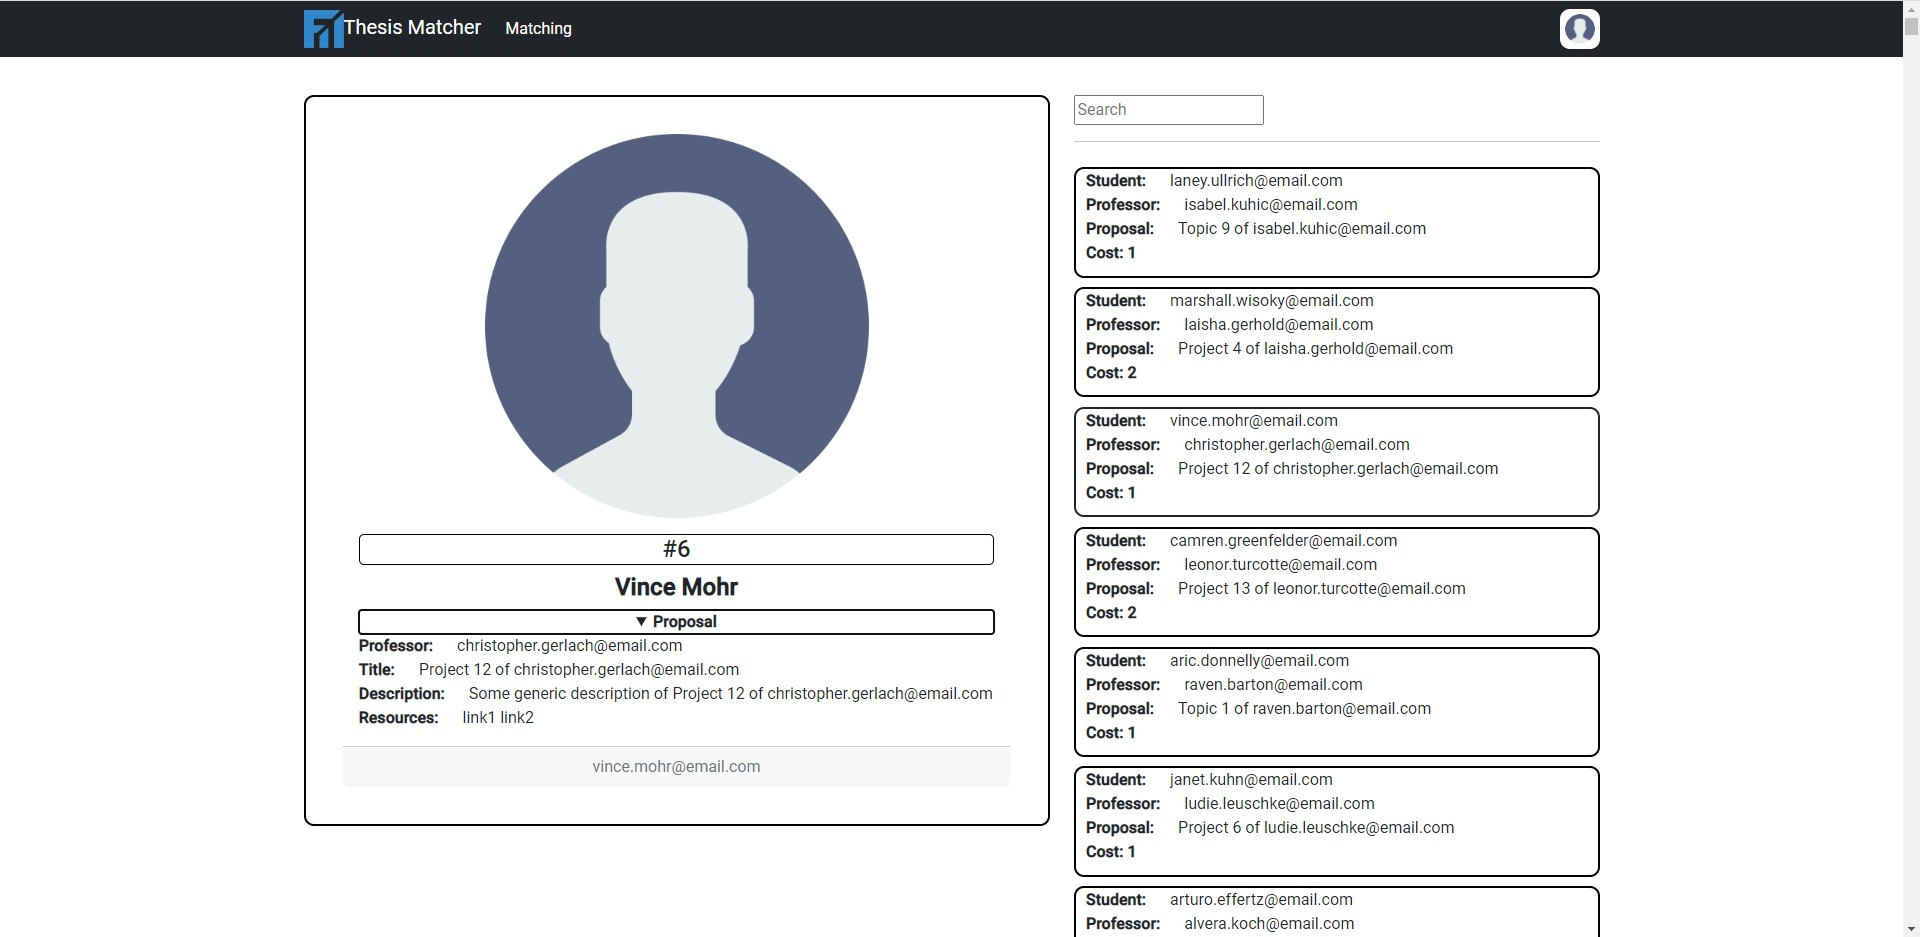
\includegraphics[width=1\textwidth, center]{matching-page.jpg}
	\caption{Matching (repartiția)}
\end{figure}

Aici se poate observa lista tuturor studenților și propunerea (proiectul sau tematica) asignată fiecăruia în funcție de preferințele sale. De asemenea, pentru fiecare asignare este înregistrat un \textit{cost} care indică locul propunerii primite în ordinea preferințelor sale (de exemplu, o asignare cu costul 1 înseamnă că propunerea a fost pe primul loc în lista sa, o alta cu costul 2 a fost pe al doilea loc etc.). În plus, există o opțiune de a căuta prin rezultat după numele studentului, al profesorului sau titlul lucrării.

Totuși, opțiunile utilizatorului sunt mult restrânse, lucru ce se poate observa și din bara de navigare, el fiind nevoit să se autentifice.

Pagina de autentificare este simplă, utilizatorul fiind nevoit să introducă email-ul și parola unui cont existent după cum se poate obeserva în figura următoare.

\begin{figure}[H]
	\centering
	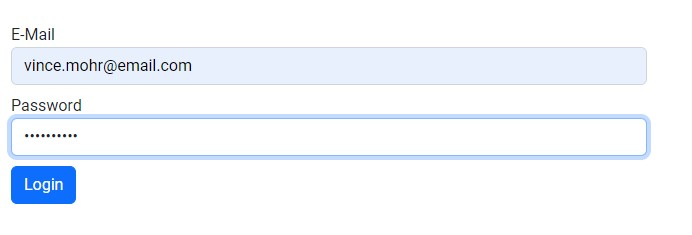
\includegraphics[width=0.5\textwidth, center]{auth-page.jpg}
	\caption{Pagina de autentificare}
\end{figure}

Odată autentificat, utilizatorul își poate schimba fotografia de profil, descrierea în care poate specifica domeniile de interes. În plus, acesta își poate schimba parola de la cont. Toate aceste setări pot fi efectuate din pagina \textbf{My Profile}.

\begin{figure}[H]
	\centering
	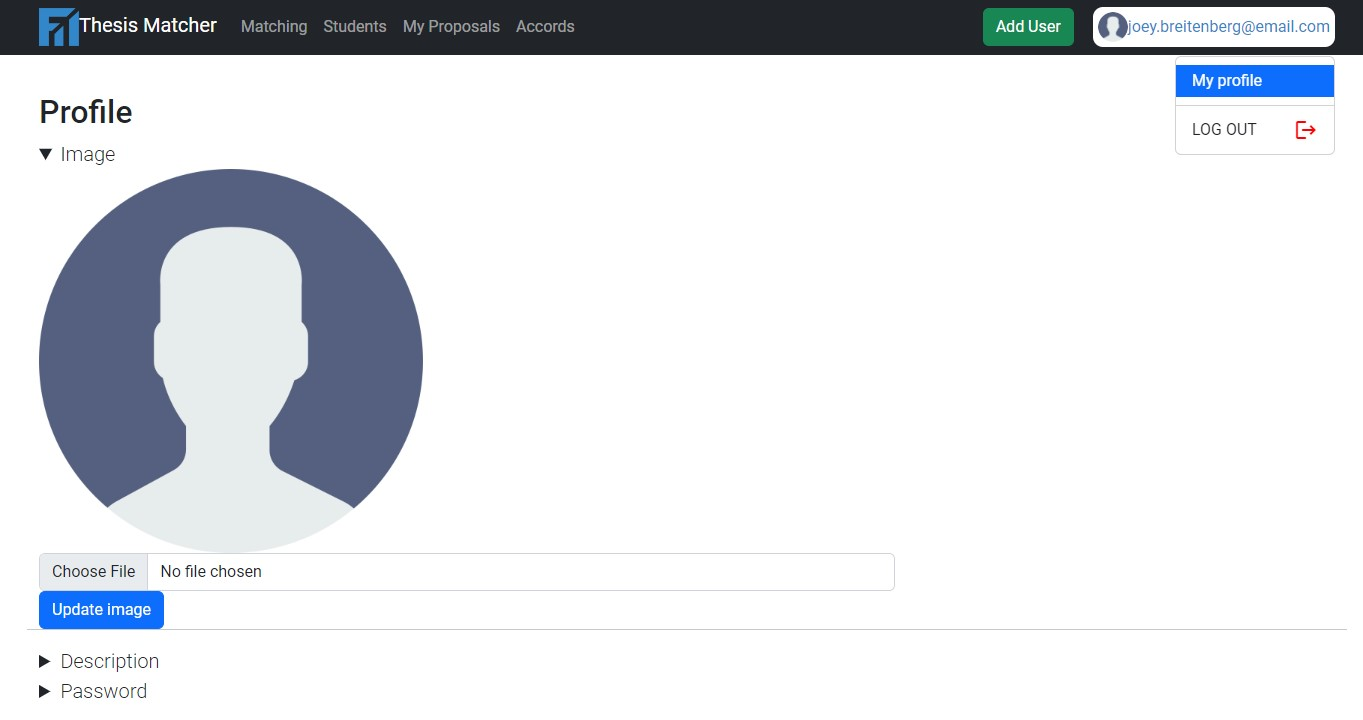
\includegraphics[width=0.5\textwidth, center]{my-profile-page.jpg}
	\caption{Profilul utilizatorului}
\end{figure}

\subsection{Interfața studentului}

Un utilizator de tip \textit{student} poate accesa pagina \textbf{Professors} unde poate vedea detalii despre fiecare profesor, însă principalul scop al acestei pagini este de a accesa propunerile fiecărui profesor în parte.

\begin{figure}[H]
	\centering
	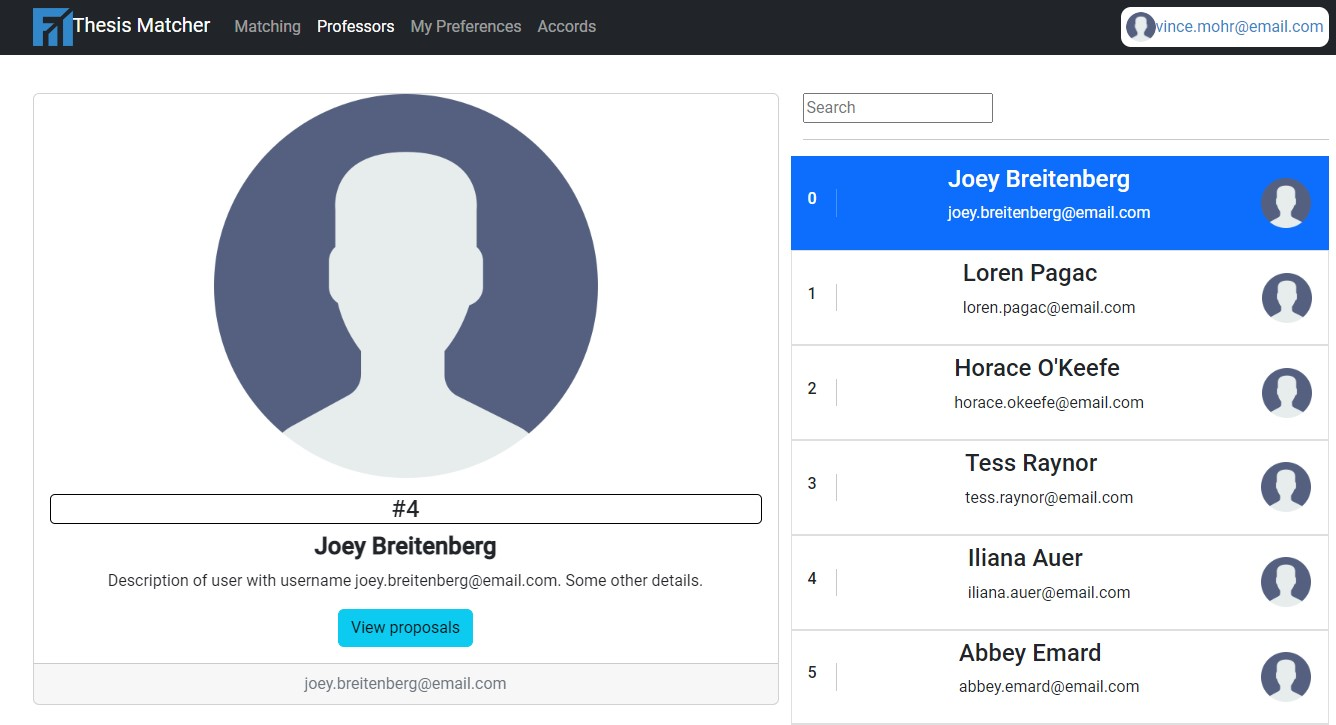
\includegraphics[width=0.5\textwidth, center]{professors-page.jpg}
	\caption{Profesorii}
\end{figure}

\begin{figure}[H]
	\centering
	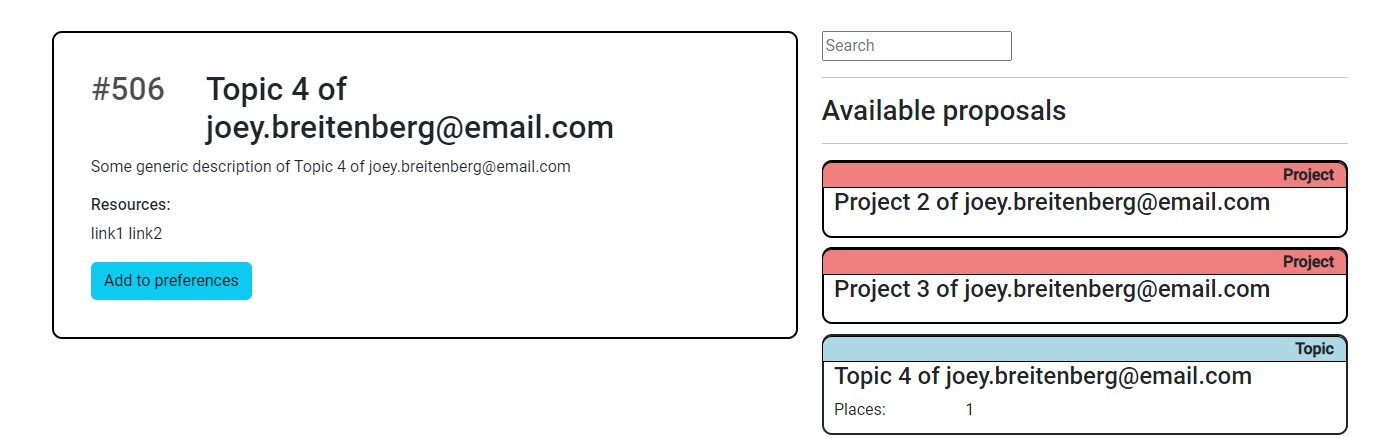
\includegraphics[width=0.5\textwidth, center]{proposals-page.jpg}
	\caption{Propunerile unui profesor}
\end{figure}

Acest lucru permite adăugarea unei propuneri la lista sa de preferințe. El poate căuta în lista de propuneri a profesorului respectiv după titlu sau descriere. Pentru a marca și diferenția opțiunile între ele după tip, proiectele au fost colorate cu roșu, iar tematicile (topics) în albastru, acestea având specificat și un număr limită de locuri disponibile, spre deosebire de proiecte care au câte unul singur. 

Pagina preferințelor (\textbf{Preferences}) conține toate propunerile apreciate de către student. Acesta poate elimina de exemplu un proiect din listă sau poate modifica rating-ul, un număr întreg între 1 și 100. După cum a fost deja menționat, două preferințe pot avea același rating, iar acest număr este utilizat strict pentru ordonarea preferințelor. Atunci când este adăugată o preferință, aceasta are inițializat rating-ul cu 1, fiind la finalul ierarhiei.

\begin{figure}[H]
	\centering
	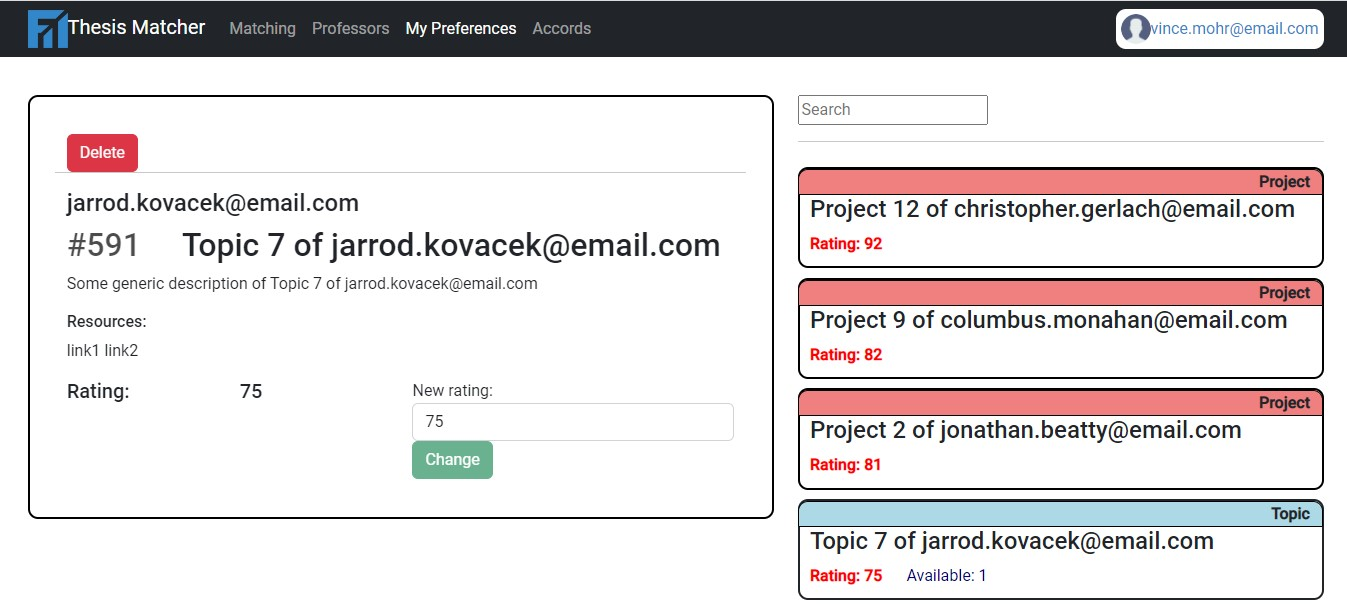
\includegraphics[width=0.6\textwidth, center]{preferences-page.jpg}
	\caption{Preferințele}
\end{figure}

\subsection{Interfața profesorului}

Interfața unui profesor este în mare măsură similară. În pagina \textbf{Students} el poate vedea o listă de studenți și iniția un acord pentru o anumită lucrare, adică să asigneze un proiect sau o tematică unui student.

Pagina \textbf{My proposals} cuprinde propunerile create de profesor. Acesta poate adăuga noi proiecte, modifica elemente deja existente sau să le elimine.

\begin{figure}[H]
	\centering
	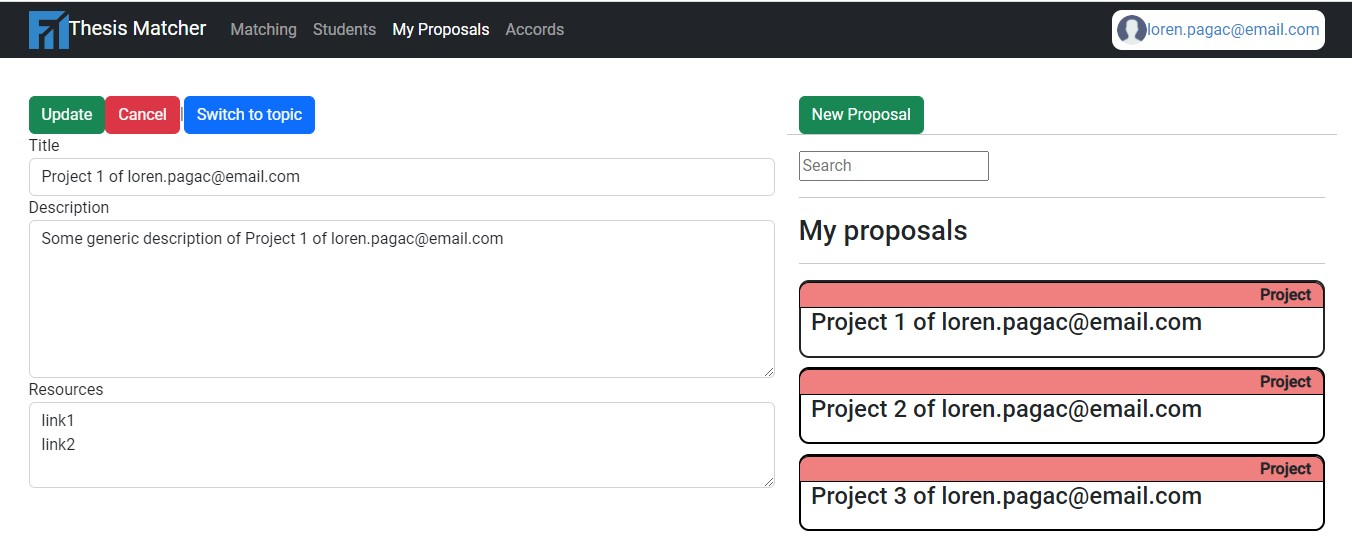
\includegraphics[width=0.6\textwidth, center]{professor-proposals-page.jpg}
	\caption{Propunerile}
\end{figure}

În secțiunea \textbf{Accords} există toate acordurile inițiate de către profesor. Pentru a fi luat în calcul, un acord trebuie însa acceptat de către student. În acest fel, studentului i se asignează deja un proiect, iar în acest fel atât acesta, cât și propunerea, nu mai intră în pasul de determinare a unei repartizări. Acordurile acceptate sunt marcate cu verde, în caz contrar, cu roșu.

\begin{figure}[H]
	\centering
	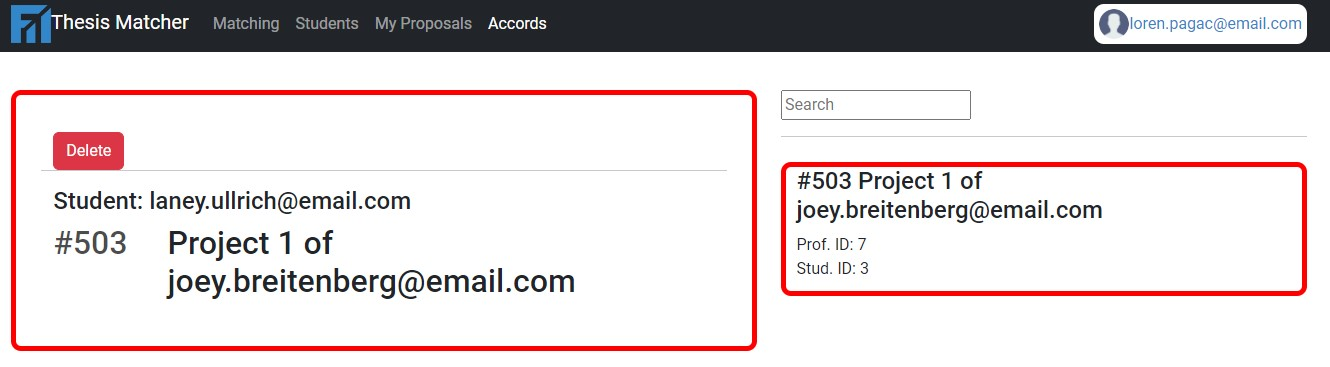
\includegraphics[width=0.6\textwidth, center]{accords-page.jpg}
	\caption{Acordurile}
\end{figure}

\subsection{Administratorul}

În cadrul acestei aplicații, fiind proiectată ca utilitar de uz intern, doar utilizatorii cu drepturi de administrator (ROLE\_ADMIN) pot adăuga noi utilizatori. Prin urmare, doar aceștia au acces la pagina \textbf{Add User} de unde pot realiza acest lucru.

\begin{figure}[H]
	\centering
	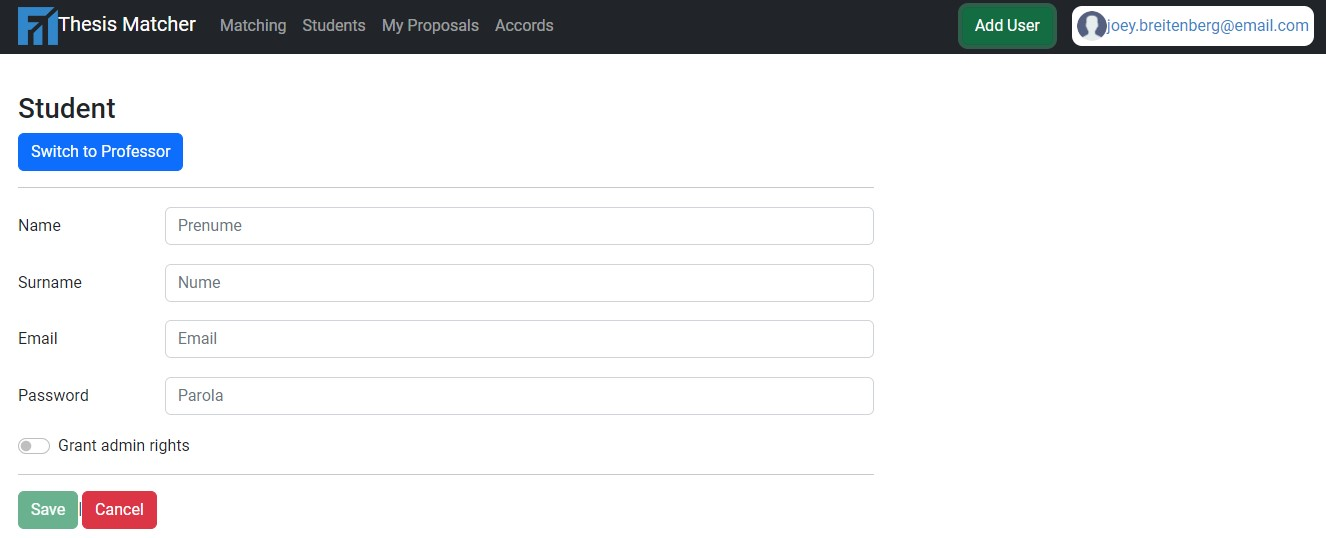
\includegraphics[width=0.6\textwidth, center]{add-user-page.jpg}
	\caption{Adăugarea unui utilizator}
\end{figure}

\section{Detalii de implementare}

Înainte de a prezenta implementarea generală a părții de front-end, este necesară explicarea alcătuirii unei componente Angular.

Componenetele sunt elementele de bază ale interfeței unei aplicații Angular, o astfel de aplicație conține un arbore de componente \cite{component1}. Acestea sunt de fapt din puct de vedere tehnic un tip de directive, întotdeauna asociate cu un template.

O componentă este alcătuită dintr-un fișier Typescript ce modelează componenta prin intermediul unei clase, un \textit{template} (șablon) ce descrie cum este construită (\textit{rendered}) aceasta și eventual un fișiser CSS care indică detalii de stilizare.

\subsection{Lifecylce hooks}

Fiecare componentă are un ciclu de viață (lifecycle) care începe odată cu instanțierea și afișarea acesteia, continuă cu detectarea schimbărilor în view și în proprietățile instanței și se termină cu distrugerea componentei și eliminarea acesteia din DOM \cite{angular-lifecycle}.

Există posibilitatea de a răspunde la astfel de evenimente din ciclul de viață al unei componente prin intermediul unor interfețe precum OnInit sau OnDestroy.

\begin{figure}[H]
	\centering
	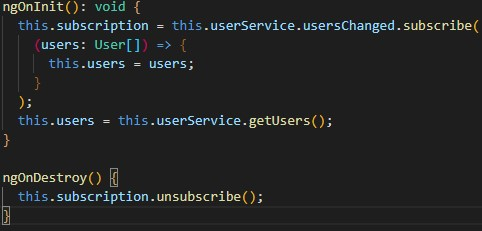
\includegraphics[width=0.6\textwidth, center]{user-list-on-init.jpg}
	\caption{Metodele ngOnInit și ngOnDestroy în componenta UserList}
\end{figure}

Se poate observa cum în metoda \texttt{ngOnInit} a componentei \texttt{UserList} sunt efectuate operații necesare instanțierii și afișării listei de utilizatori. Utilizând serviciul \texttt{userService} injectat în constructor, se crează un obiect de tipul \texttt{Subscription} pentru a obține un tablou de utilizatori. În metoda \texttt{ngOnDestroy}, acest obiect este înlăturat pentru a optimiza folosirea memoriei.

\subsection{Accesarea unei rute}

Angular este utilizat în principal pentru crearea de aplicații \textit{single-page}, adică toate funcționalitățile există într-o singură pagină HTML. Browser-ul încarcă doar părțile (componentele) necesare utilizatorului, fără a încărca o nouă pagină. De aceea, utilizatorul navighează prin intermediul rutelor predeterminate \cite{angular-routes}. Acestea permit afișarea unor view-uri specifice în funcție de calea URL. Pentru a dispune de această funcționalitate, trebuie importat modulul \texttt{RouterModule} din pachetul \texttt{@angular/router}.

Rutele sunt stabilite în acest caz în modulul \texttt{AppRoutingModule}, iar definiția unei rute este din punct de vedere tehnic un obiect JavaScript \cite{angular-routes}. Fiecare are măcar proprietățile \texttt{path} ce indică calea URL și \texttt{component}, numele componentei afișate. Definirea este realizată în manieră ierarhică, fiecare rută putând avea o listă de descendenți. Spre exemplu, în imaginea următoare se poate vedea rutele necesare vizualizării propunerilor, a detaliilor unui anumit element, adăugarea și modificarea unei propuneri.

\begin{figure}[H]
	\centering
	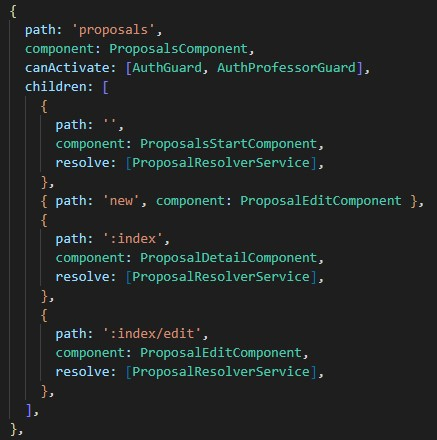
\includegraphics[width=0.5\textwidth, center]{proposals-routes.jpg}
	\caption{Rutele pentru propuneri}
\end{figure}

\subsection{Serviciile}

În cadrul acestei aplicații, serviciile sunt o parte esențială în special în comunicarea dintre componente și transmiterea și primirea de informații către/de la back-end. Fiecare serviciu este adnotat cu \texttt{Injectable} pentru a permite injectarea acestora în alte obiecte.

În figura următoare este prezentată parțial implementarea serviciului de autentificare.

\begin{figure}[H]
	\centering
	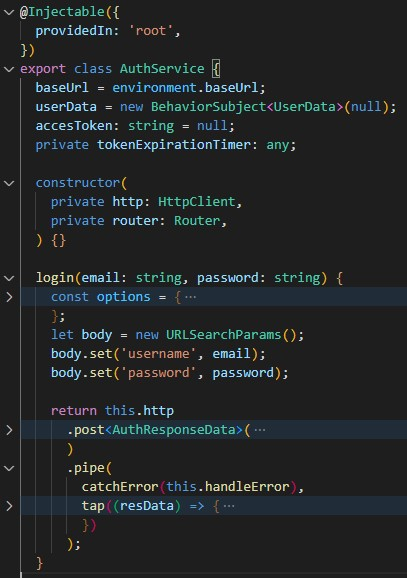
\includegraphics[width=0.4\textwidth, center]{auth-service.jpg}
	\caption{Serviciul de autentificare}
\end{figure}

Acesta utilizează la rândul său serviciile \texttt{HttpClient} pentru comunicarea cu back-end-ul prin request-uri HTML și \texttt{Router} pentru navigare. Astfel, în metoda \texttt{login} este efectuat un request \texttt{POST}, cu \textit{body} de tipul \texttt{x-www-form-urlencoded} (specificat în \textit{headers}) conținând câmpurile \textit{username} și \textit{password} cu valorile aferente. Rezultatul acestui request este un obiect de tipul \textit{AuthResponseData} ce conține în special câmpul \textit{accessToken}. Acest token este un șir de caracter reprezentând un JWT (JSON Web Token) și este unic fiecărui utilizator și necesar pentru efectuarea cu succes a oricărui request ulterior.

Un alt detaliu este reprezentat de variabila \texttt{userData}, de tipul \textit{BehaviourSubject<UserData>}, care permite emiterea unor evenimente pentru a indica autentificarea și dezautentificarea utilizatorului.

\subsubsection{Resolver}

Un categorie particulară a serviciilor este cea de \textbf{Resolvers}. Un astfel de serviciu implementează interfața \textit{Resolve} și este utilizat pentru operații premergătoare încărcării unei componente, iar specificarea acestui are loc în \texttt{AppRoutingModule}. În cazul propunerilor, prin intermediu serviciului \texttt{ProposalService} este obținută o listă completă a propunerilor profesorului autentificat.

\begin{figure}[H]
	\centering
	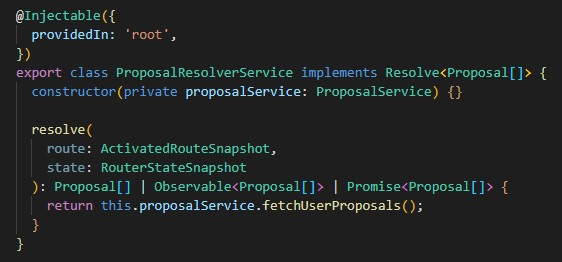
\includegraphics[width=0.5\textwidth, center]{proposal-resolver.jpg}
	\caption{Resolver pentru propuneri}
\end{figure}

\subsubsection{Guard}

O altă categorie este cea a gărzilor sau \textbf{Guards} în engleză, care autorizează accesul utilizatorilor la diversele rute în conformitate cu drepturile acestora, de student și profesor sau administator. În \texttt{AuthGuard} este detaliată verificarea dacă utlizatorul este autentificat. În cazul favorabil, acestuia îi este permis accesul la ruta respectivă prin returnarea valorii \textit{true}, altfel este returnat un obiect de tipul textit{UrlTree} pentru a îl redirecționa spre autentificare.

\begin{figure}[H]
	\centering
	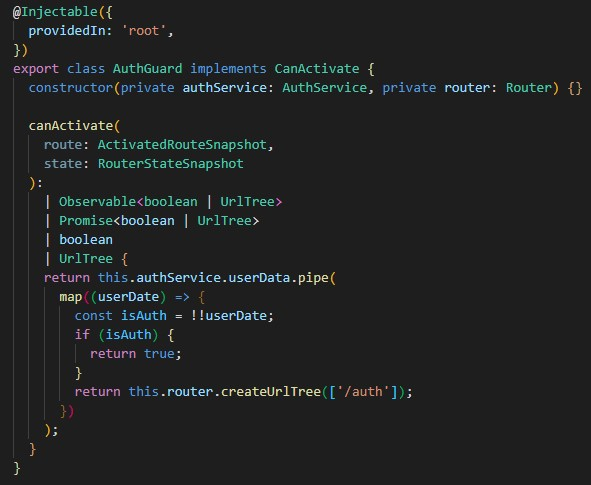
\includegraphics[width=0.5\textwidth, center]{auth-guard.jpg}
	\caption{Guard pentru autentificare}
\end{figure}

\subsection{Formularele}

Obținerea, modificarea și ștergerea datelor nu ar fi posibilă fără formularele utilizate. În cadrul acestei aplicații, pe parte de front-end a fost aleasă metoda \textit{template-driven} de implementare a formularelor (forms). Un astfel de tip folosește \textit{two-way data binding} pentru a actualiza modelul de date din componentă în timp ce au loc modificări și vice-versa \cite{angular-td-forms}.

\begin{figure}[H]
	\centering
	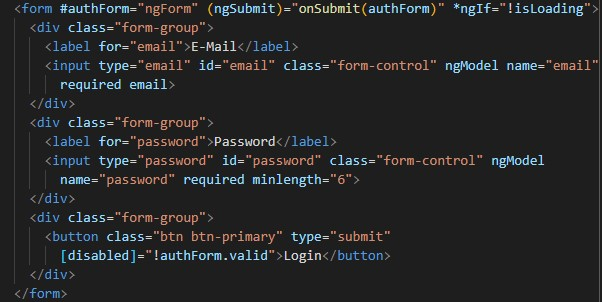
\includegraphics[width=0.6\textwidth, center]{auth-form.jpg}
	\caption{Formular de autentificare}
\end{figure}

Se poate observa cum formularul de autentificare este compus din mai multe input-uri, cel pentru email și cel pentru parolă, incluse în div-uri marcate de clasa \textit{form-group}. Fiecare input are o serie de directive specifice ce asigură restricții necesare pentru o bună experiență a utlizatorului. De exemplu, directiva \texttt{required} indică obligativitatea completării input-ului, iar \texttt{email} verifică forma corectă a email-ului.

Procesarea datelor are loc pe în codul de Typescript odată ce formularul este trimis, în acel moment fiind apelată metoda \texttt{OnSubmit} ce primește ca argument un obiect de tipul \textit{Form}.

\section{Precizări}

Versiunea de Angular utilizată este 13.

În primul rând, pentru stilizarea șabloanelor (templates) componentelor a fost folosit Bootstrap v5.2. Acest framework a permis facilitarea poziționării elementelor HTML, modificarea stilului și dimensiunilor acestora.

Căile URL necesare request-urilor către back-end au fost construite utilizând enum \textit{ApiPaths} definit în fișiserul \texttt{environment.ts}.

Pentru modelarea ușoară a obiectelor JSON în comunicarea cu back-end au fost create clase \textit{model} precum \textit{ProposalModel}, \textit{PreferenceModel} etc.